\documentclass[UTF8]{ctexart}
\usepackage{anyfontsize}
\usepackage{geometry}
    \geometry{left=4cm,right=4cm,top=2cm,bottom=2cm}
\usepackage{amsmath, amssymb, amsthm}
\usepackage{caption} 	 % 标题
\usepackage{xcolor} 	 % 颜色
\usepackage{graphicx} 	 % 引用图片
\usepackage{float}
\usepackage{framed} 	 % 方框 \begin{framed}
\usepackage{indentfirst} 	 % 首行缩进 
    \setlength{\parindent}{0em}
\usepackage{setspace} 	 % 行间距 \begin{spacing}{arg}
\usepackage{extarrows} 	 % 箭头宏包 \xLongrightarrow 
\usepackage{esvect} 	 % 向量箭头 \vv{}
\usepackage{siunitx} 	 % 国际单位 \si{unit} \SI{number}{unit} 
\usepackage{esint} 	 % 积分符号
\usepackage{mathrsfs}

% font
\newcommand{\ve}[1]{\boldsymbol{\mathbf{#1}}}
\newcommand{\unit}[1]{\boldsymbol{\mathbf{\hat{#1}}}}
\newcommand{\mcal}{\mathcal}
\newcommand{\mscr}{\mathscr}
% common symbol
\newcommand{\E}{\mathrm e}
\renewcommand{\I}{\mathrm i}
\newcommand{\R}{\mathbb R}
\newcommand{\Z}{\mathbb Z}
\newcommand{\N}{\mathbb N}
\newcommand{\Q}{\mathbb Q}
\newcommand{\C}{\mathbb C}
% differentiation
\def \DD #1.#2.#3 {\dfrac{d^{#1} #2}{d #3^{#1}}}
\def \PP #1.#2.#3 {\dfrac{\partial^{#1} #2}{\partial #3^{#1}}}
\def \dd #1.#2 {\dfrac{d #1}{d #2}}
\def \pp #1.#2 {\dfrac{\partial #1}{\partial #2}} 
% matrix
\newcommand{\transp}{^{\top}}
\DeclareMathOperator{\tr}{tr}

\pagestyle{empty}

\begin{document}
\section{常用积分表}
注: 常数 $ C $ 省略.

\subsection{基本}
$\displaystyle d x = \dfrac{d(ax + b)}{a} \hspace{5em} \int f(ax + b) \,dx = \dfrac{1}{a} \int f(ax + b) \,d(ax + b) $

\subsection{有理函数}
 
$\displaystyle
\int \dfrac{1}{ax^2 + bx + c} \,dx =  \begin{cases}
\dfrac{2}{\sqrt{-\Delta}} \arctan \dfrac{ax + b}{\sqrt{-\Delta}} \qquad, \Delta < 0 \\[1em]
\dfrac{1}{\sqrt{\Delta}} \ln \left| \dfrac{x - x_1}{x - x_2} \right| = \dfrac{1}{|a|(x_1 - x_2)} \ln \left| \dfrac{x - x_1}{x - x_2} \right|  \qquad, \Delta > 0, x_1 > x_2
\end{cases} 
$
\vskip 1em
$\displaystyle \int \frac{x}{ax^2 + bx + c}\,dx = \frac{1}{2a} \ln \left| ax^2 + bx + c \right| - \frac{b}{2a} \int \frac{dx}{ax^2 + bx + c}  $

\subsection{无理函数/反三角函数}
$\displaystyle \int \dfrac{1}{a^2 + x^2} \,dx = \dfrac{1}{a}\arctan \dfrac{x}{a} $
\hskip 4em
$\displaystyle \int \dfrac{1}{\sqrt{a^2 - x^2}} \,dx = \arcsin \dfrac{x}{a} $
\vskip 1em

$\displaystyle \int \dfrac{1}{\sqrt{x^2 \pm a^2}} \,dx = \ln \left|x + \sqrt{x^2 \pm a^2}\right|  $


\subsection{三角函数积分/导数}
$ (\tan x)' = \sec^2 x \qquad (\cot x)' = -\csc^2 \qquad (\sec x)' = \sec x \tan x \qquad (\csc x)' = - \csc x \cot x $
\vskip 1em

$\displaystyle \int \tan x \,dx = - \ln |\cos x| $, $\quad$ ($ \tan $ 分母为 $ \cos $)
\vskip 1em

$\displaystyle \int \cot x \,dx = \ln |\sin x| $, $\quad$ ($ \cot $ 分母为 $ \sin $)
\vskip 1em

$\displaystyle \int \sec x \,dx = \ln |\sec x + \tan x| $
\vskip 1em

$\displaystyle \int \csc x \,dx = \ln |\csc x - \cot x| $

\subsection{其它}
$\displaystyle \int f(x) \E^x \,dx = \E^x \big[ f(x) - f'(x) + f''(x) - f'''(x) + f^{(4)}(x) - \cdots \big] $
\vskip 1em

$\displaystyle \int f(x) \E^{-x} \,dx = - \E^{-x} \big[ f(x) + f'(x) + f''(x) + f'''(x) + f^{(4)}(x) + \cdots \big]  $



\subsection{竖线记号}
\begin{itemize}
    \item 线性: $ \big[ C \cdot f(x) \big]_a^b = C \cdot \big[ f(x) \big]_a^b \hspace{3em} \big[f(x) \pm g(x) \big]_a^b = \big[f(x)\big]_a^b \pm \big[g(x) \big]_a^b $
    \item $ -\big[f(x)\big]_a^b = \big[-f(x)\big]_a^b = \big[f(x)\big]_b^a $
\end{itemize}



\newpage
\section{积分技巧}
\subsection{定积分}
\begin{enumerate}
    \item $ f(x) $ 为奇函数: \[ \int_{-a}^{a} f(x) \,dx = 0 \]
    \item $ f(x) $ 为偶函数: \[ \int_{-a}^{a} f(x) \,dx = 2 \int_{0}^{a} f(x) \,dx \]
    \item 三角函数: \[ \int_{0}^{\pi/2} f(\sin x) \,dx = \int_{0}^{\pi / 2} f(\cos x) \,dx \]\[ \int_{0}^{\pi} x f(\sin x) \,dx = \dfrac{\pi}{2} \int_{0}^{\pi} f(\sin x) \,dx \]
    \item 周期函数: $ f(x) $ 的周期为 $ T $, 区间 $ I = [0, T] $, 将 $ I $ 平移得到 $ I + a = [a, a + T] $: \[ \int_I f(x) \,dx = \int_{I + a} f(x) \,dx \]
    \item Wallis' Integral: \[ \int_{0}^{\pi/2} \sin^n x \,dx = \int_{0}^{\pi/2} \cos^n x \,dx = \begin{cases}
        \dfrac{n - 1}{n} \cdot \dfrac{n - 3}{n - 2} \cdots \dfrac{1}{2} \cdot \dfrac{\pi}{2} = \dfrac{(n - 1)!!}{n!!}\cdot \dfrac{\pi}{2} &, n \text{ 为偶数} \\[1em]
        \dfrac{n - 1}{n} \cdot \dfrac{n - 3}{n - 2} \cdots \dfrac{4}{5} \cdot \dfrac{2}{3} = \dfrac{(n - 1)!!}{n!!} &, n \text{ 为奇数}
    \end{cases} \]
    \item 与求和 $ (\sum) $ 类似的积分区间平移: \[ \int_{I} f(x) \,dx = \int_{I \pm k} f(x \mp k) \,dx \]
\end{enumerate}  

\vskip 2em
\subsubsection{对称性}
定义域关于原点对称, $ f(x) $ 和 $ f(-x) $ 积分相同:
\[ \int_{-a}^{a} f(x) \,dx = \int_{-a}^{a} f(-x) \,dx \tag{*}\]

所以有:
\[ \int_{-a}^{a} f(x) \,dx = \int_{-a}^{a} \dfrac{f(x) + f(-x)}{2} \,dx = \int_{0}^{a} \big[ f(x) + f(-x) \big] \,dx  \]
注意 $ f(x) + f(-x) $ 为偶函数.
\vskip 2em

可将 $ (*) $ 推广至任意区间:
\[ \int_{a}^{b} f(x) \,dx = \int_{a}^{b} (a + b - x) \,dx \]

\begin{figure}[H]
    \centering
    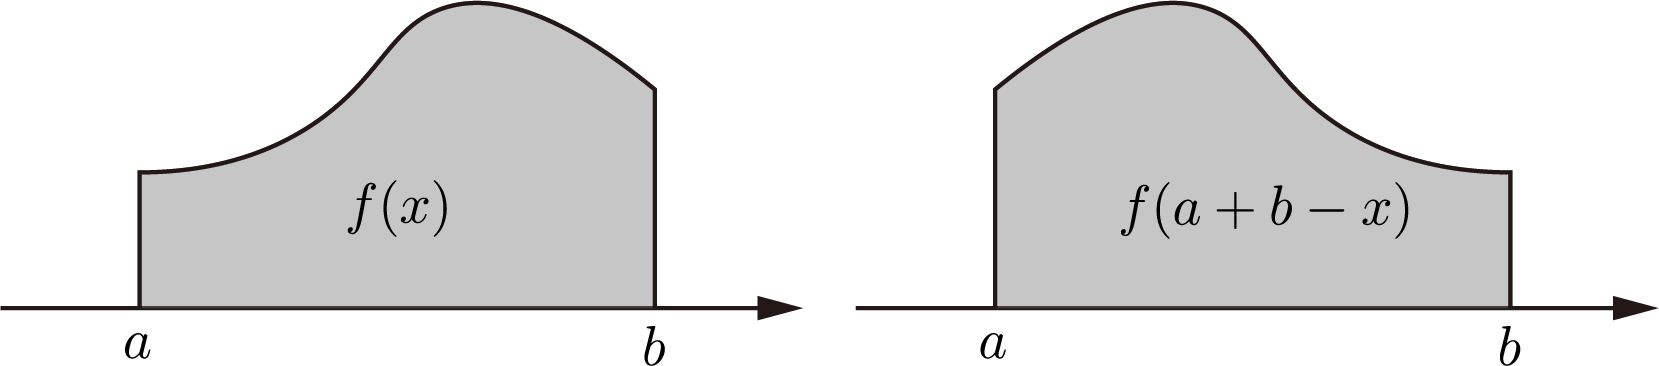
\includegraphics[width = 0.8\linewidth]{symmetry1}
\end{figure} 


应用:
\[ \int_{0}^{r} x^m (r - x)^n \,dx = \int_{0}^{r} x^n (r - x)^m \,dx \]


\vskip 3em
\subsection{二重积分}
\begin{enumerate}
    \item 常数: \[ \displaystyle \int_D C \,dx\,dy = m(D) \]
    \item 部分可加(要求参与并集运算的两个区间互斥): \[ \int_Y \int_{X_1} f \,dx\,dy + \int_Y \int_{X_2} f \,dx\,dy = \int_Y \int_{X_1 \cup X_2} f \,dx\,dy \]\[ \int_{Y_1} \int_{X} f\,dx\,dy + \int_{Y_2}\int_{X} f\,dx\,dy = \int_{Y_1 \cup Y_2} \int_X f \,dx\,dy \] 
\end{enumerate}

\begin{figure}[H]
    \centering
    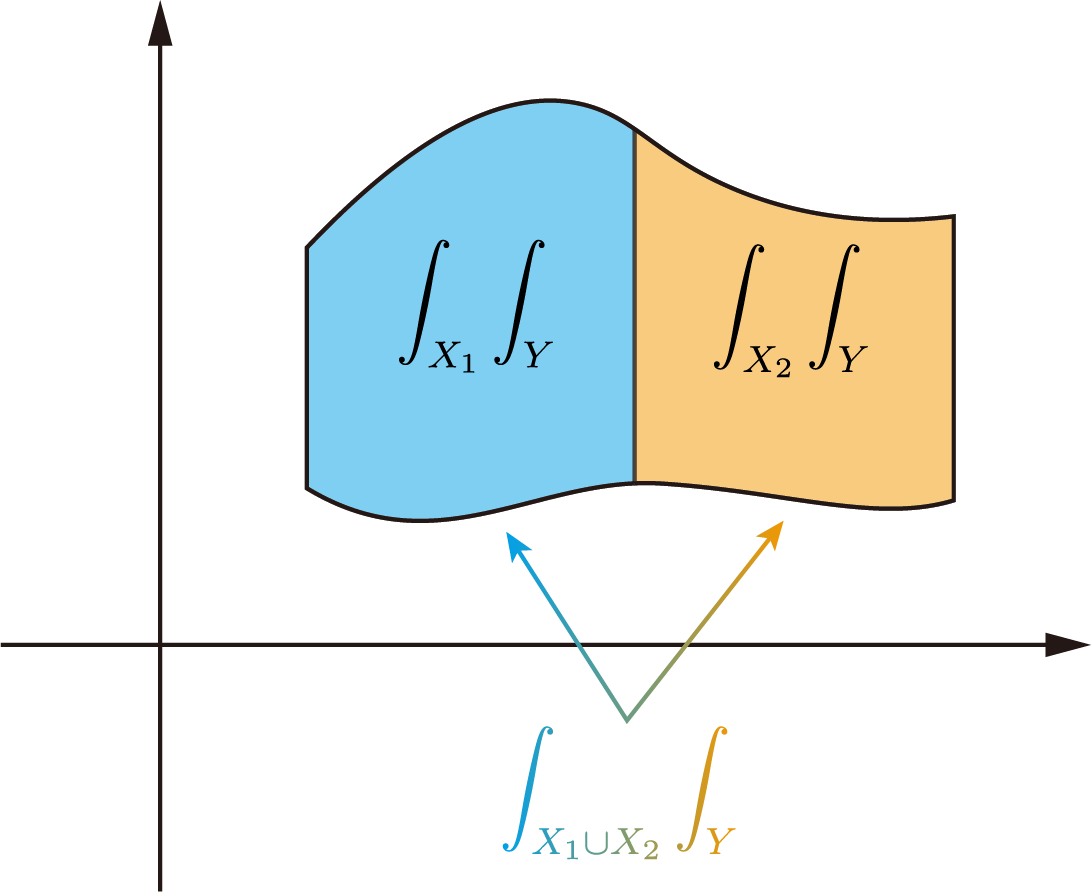
\includegraphics[width = 0.5\linewidth]{region_additive}
    \caption*{区域部分可加性图解}
\end{figure}


\subsubsection{对称性}
类似于一元函数定积分, 当区域具有对称性时, 区域上二重积分也有一定性质:

当 $ f $ 是关于 $ x $ 或 $ y $ 的奇/偶函数, 可参考一元函数定积分相关性质.

\begin{enumerate}
    \item 当定义域关于 $ x $ 轴对称, 将函数沿 $ x $ 轴面对称, 积分不变 \[ \iint_D {\color{red} f(x, y)} \,dx\,dy = \iint_D {\color{blue} f(x, -y)} \,dx\,dy \]
    \item 当定义域关于 $ y $ 轴对称, 将函数沿 $ y $ 轴面对称, 积分不变 \[ \iint_D {\color{red} f(x, y)} \,dx\,dy = \iint_D {\color{blue} f(-x, y)} \,dx\,dy \]
    \item 当定义域关于原点对称, 将函数沿原点轴对称, 积分不变 \[ \iint_D {\color{red} f(x, y)} \,dx\,dy = \iint_D {\color{blue} f(-x, -y)} \,dx\,dy \]
    \item 当定义域关于 $ y = x $ 对称, 将函数沿 $ y = x $ 面对称(交换 $x$,$y$), 积分不变 \[ \iint_D {\color{red} f(x, y)} \,dx\,dy = \iint_D {\color{blue} f(y, x)} \,dx\,dy \]
\end{enumerate}

\begin{figure}[H]
    \centering
    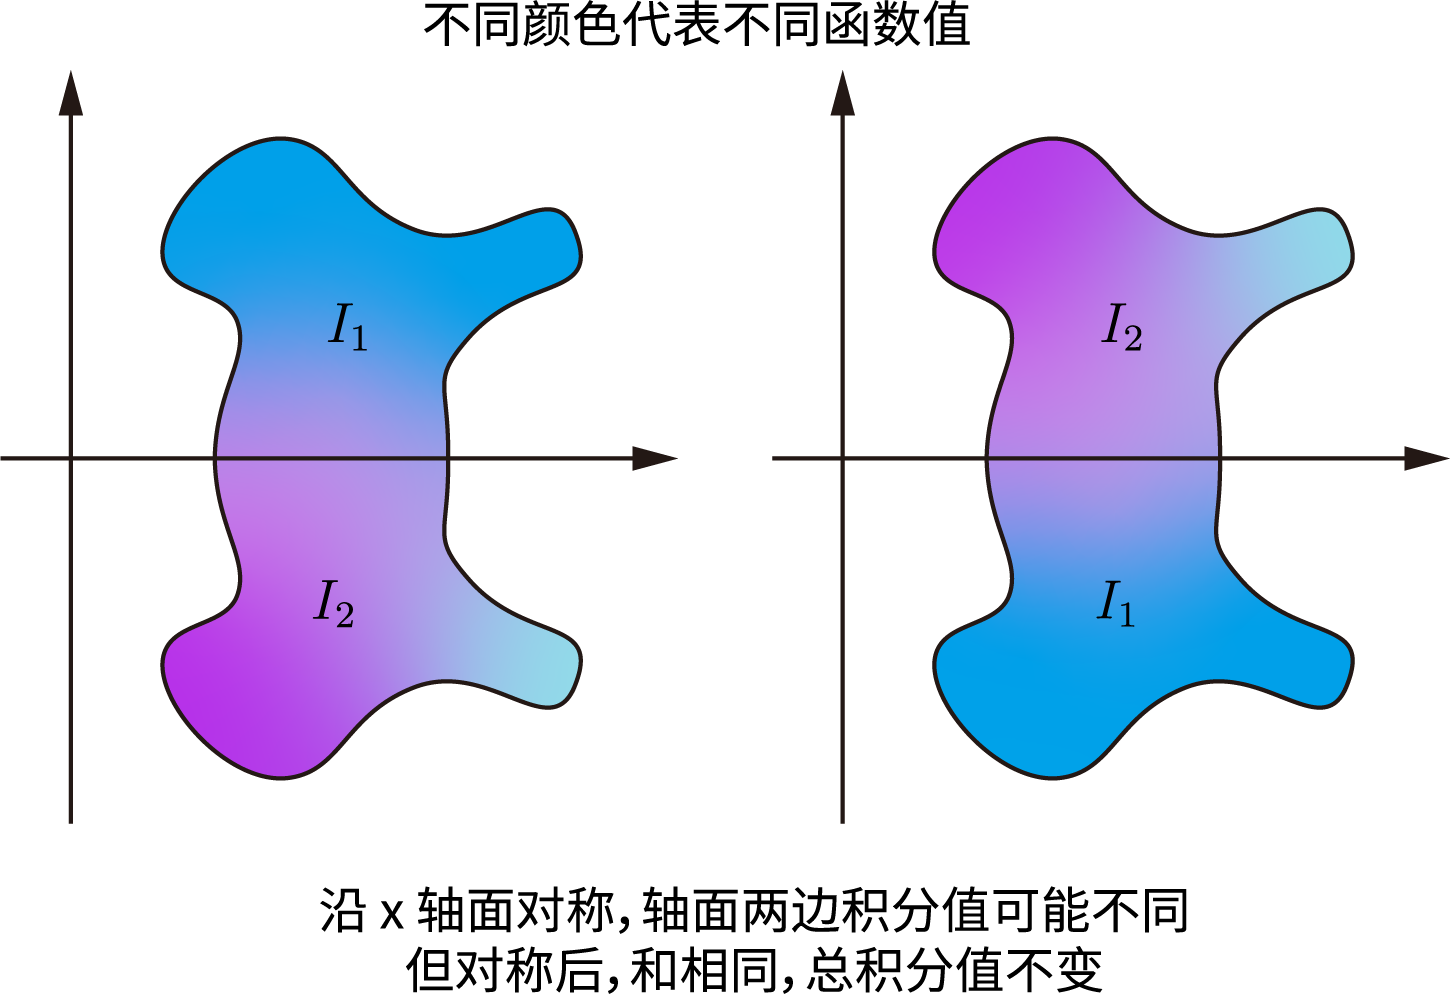
\includegraphics[width = 0.65\linewidth]{symmetry2}
\end{figure}



\end{document}